% Drawing 69/06-2 -- folder 69, batch 06, archive page 102 (PDF page 103).
% Transcription: un grand triangle de sommets $\tilde a = p(\tilde\gamma)$ (en haut), $\tilde b = q(\tilde\gamma)$ (en bas à droite), $\tilde c = r(\tilde\gamma)$ (en bas à gauche), avec en son centre un petit triangle dont les côtés portent $u$, $v$, $w$ ; chaque sommet du grand est relié au petit par un trait
% Kind: large triangle with a small central triangle. Method 2 (schematic redraw from the facsimile). Status: ok.
% Notes: Large triangle a~ = p(gamma~) (top), b~ = q(gamma~) (lower right), c~ = r(gamma~) (lower left); in its centre a small triangle whose sides carry u, v, w; each vertex of the large one joined to the small one.
% Coordinates: 1 unit = 1 mm = 1/100 of the crop width (bbox in page fractions: [0.2, 0.45, 0.62, 0.64]).
% Redrawn by Claude (claude-opus-5-5), issue #73, 2026-11-07; not checked by a human; not compiled (no TeX in the session).
% Rights: reproduces part of the work -- behind RENDER_TRANSCRIPTS, never published by itself.
\documentclass[tikz,border=3pt]{standalone}
\usepackage{amsmath,amssymb}
\usetikzlibrary{patterns,arrows.meta}
\tikzset{pencil/.style={black!45}, struck/.style={black!35}, mark/.style={circle,draw,inner sep=1.3pt}, pt/.style={circle,fill,inner sep=0.9pt}, opt/.style={circle,draw,fill=white,inner sep=1.1pt}}
\begin{document}
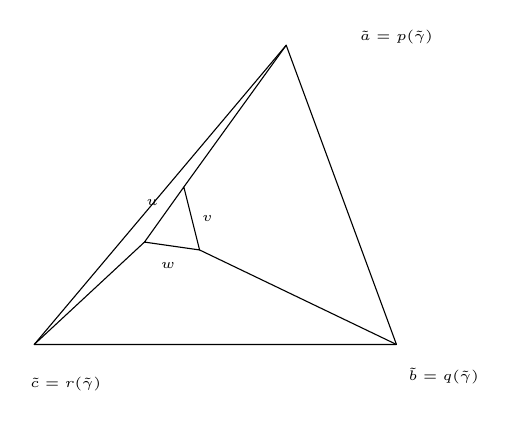
\begin{tikzpicture}[x=1mm,y=1mm,line cap=round,line join=round,font=\scriptsize]
\draw (68,-12) -- (82,-50) -- (36,-50) -- cycle;
\draw (50,-37) -- (55,-30) -- (57,-38) -- cycle;
\draw (68,-12) -- (55,-30);
\draw (82,-50) -- (57,-38);
\draw (36,-50) -- (50,-37);
\node[inner sep=1pt] at (82,-11) {\tiny $\tilde a = p(\tilde\gamma)$};
\node[inner sep=1pt] at (88,-54) {\tiny $\tilde b = q(\tilde\gamma)$};
\node[inner sep=1pt] at (40,-55) {\tiny $\tilde c = r(\tilde\gamma)$};
\node[inner sep=1pt] at (51,-32) {\tiny $u$};
\node[inner sep=1pt] at (58,-34) {\tiny $v$};
\node[inner sep=1pt] at (53,-40) {\tiny $w$};
\end{tikzpicture}
\end{document}
